%%%%%%%%%%%%%%%%%%%%%%% file template.tex %%%%%%%%%%%%%%%%%%%%%%%%%
%
% This is a general template file for the LaTeX package SVJour3
% for Springer journals.          Springer Heidelberg 2010/09/16
%
% Copy it to a new file with a new name and use it as the basis
% for your article. Delete % signs as needed.
%
% This template includes a few options for different layouts and
% content for various journals. Please consult a previous issue of
% your journal as needed.
%
%%%%%%%%%%%%%%%%%%%%%%%%%%%%%%%%%%%%%%%%%%%%%%%%%%%%%%%%%%%%%%%%%%%
%
% First comes an example EPS file -- just ignore it and
% proceed on the \documentclass line
% your LaTeX will extract the file if required
\begin{filecontents*}{example.eps}
%!PS-Adobe-3.0 EPSF-3.0
%%BoundingBox: 19 19 221 221
%%CreationDate: Mon Sep 29 1997
%%Creator: programmed by hand (JK)
%%EndComments
gsave
newpath
  20 20 moveto
  20 220 lineto
  220 220 lineto
  220 20 lineto
closepath
2 setlinewidth
gsave
  .4 setgray fill
grestore
stroke
grestore
\end{filecontents*}
%

\RequirePackage{fix-cm}
%
%\documentclass{svjour3}                     % onecolumn (standard format)
%\documentclass[smallcondensed]{svjour3}     % onecolumn (ditto)
\documentclass[twocolumn]{svjour3}       % onecolumn (second format)
%\documentclass[twocolumn]{svjour3}          % twocolumn
%
\smartqed  % flush right qed marks, e.g. at end of proof
%
\usepackage{color}
\usepackage{multirow}
\usepackage[usenames,dvipsnames,svgnames,table]{xcolor}
\usepackage{booktabs}
\usepackage{tabu,xcolor,colortbl}
\usepackage{rotating}
\usepackage{amsmath,array}    
\usepackage[utf8]{inputenc} 
\DeclareUnicodeCharacter{FB01}{fi} %Caracter especial
\usepackage{graphicx} %Imagens
\usepackage{listings} % Codes
\usepackage{tabularx} % in the preamble
\usepackage{mathtools} % Serve para as equacoes
\usepackage{cite}


\usepackage{hyphenat}
\usepackage[english]{babel}
\hyphenation{ef-fect-ive consi-de-red demons-trate se-cond veri-fication covera-ge des-cribe reali-zation opera-tor re-pre-sentation methodo-lo-gy di-gi-tal chara-cteristics granu-lar ge-nerally diago-nal para-meters spe-cification re-presentable me-thods ope-rations sche-dule deve-loped des-cribes diffe-rent mo-dels sa-ving ve-rified proper-ties mini-mum mathe-matical tole-rated limi-ted op-tical net-works semi-conduc-tor go-to-pro-grams }

\newcommand{\head}[1]{\textnormal{\textbf{#1}}}
\renewcommand{\lstlistingname}{Algorithm}
\renewcommand{\arraystretch}{1.3}
\usepackage[table]{xcolor}
\usepackage{color}
\definecolor{dkgreen}{rgb}{0,0.6,0}
\definecolor{gray}{rgb}{0.5,0.5,0.5}
\definecolor{mauve}{rgb}{0.58,0,0.82}
\definecolor{Gray}{gray}{0.93}
\definecolor{DarkGray}{gray}{0.70}

\lstset{frame=tb,
  language=c,
  aboveskip=3mm,
  belowskip=3mm,
  showstringspaces=false,
  columns=flexible,
  basicstyle={\small\ttfamily},
  numbers=none,
  numberstyle=\tiny\color{gray},
  keywordstyle=\color{black},
  commentstyle=\color{dkgreen},
  stringstyle=\color{mauve},
  breaklines=true,
  breakatwhitespace=true,
  tabsize=3
}
\DeclareGraphicsExtensions{.pdf,.png,.jpg}
%
% \usepackage{mathptmx}      % use Times fonts if available on your TeX system
%
% insert here the call for the packages your document requires
%\usepackage{latexsym}
% etc.
%
% please place your own definitions here and don't use \def but
% \newcommand{}{}
%
% Insert the name of "your journal" with
% \journalname{myjournal}
%

\renewcommand{\baselinestretch}{0.96}

\newcommand{\comment}[1]{}

\begin{document}
\title{Applying Multi-Core Model Checking to Hardware-Software Partitioning in Embedded Systems}
\author{Alessandro Trindade\and Hussama Ismail\and Renato Degelo\and Edilson Galv\~ao\and Helder Silva \and Lucas Cordeiro}

\institute{A. Trindade, H. Ismail, R. Degelo, E. Galv\~ao \at
              Graduate Program in Electrical Engineering, Federal University of Amazonas, Brazil \\
%              Tel.: +123-45-678910\\
%              Fax: +123-45-678910\\
              \email{\{alessandro.b.trindade, hussamaismail, rdegelo, esj.galvao\}@gmail.com}          %  \\
%             \emph{Present address:} of F. Author  %  if needed
           \and
           H. Silva and L. Cordeiro \at
              Federal University of Amazonas, Brazil
              \email: prhsilva2012@gmail.com lucascordeiro@ufam.edu.br           %  \\
}

\maketitle

\begin{abstract}
We present an alternative approach to solve the hardware (HW) and software (SW) partitioning problem, which uses Bounded Model Checking (BMC) based on Satisfiability Modulo Theories (SMT) in conjunction with a multi-core support using Open MultiProcessing. The multi-core SMT-based BMC approach allows initializing many verification instances based on the number of available processing cores. Each instance checks for a different optimum value until the optimization problem is satisfied. The goal is to show that multi-core model-checking techniques can be effective, in particular cases, to find the optimal solution of the HW-SW partitioning problem using an SMT-based BMC approach. 
We implement and evaluate our algorithms on top of the Efficient SMT-Based Context-Bounded Model Checker (ESBMC). We also compare our approaches to other state-of-the-art optimization tools: Matlab and Z3. Experimental results show that no single optimization tool solves all benchmarks; however, Matlab and Z3 are the most efficient ones to solve HW-SW partitioning problems, although ESBMC had a significant performance improvement from its sequential to parallel version.
\end{abstract}

\keywords{hardware-software co-design \and hardware-software partitioning\and optimization\and model checking\and multi-core\and OpenMP }

%---------------------------------
\section{Introduction}
\label{Introduction}
%---------------------------------

Nowadays, with the strong development of embedded systems, the design phase plays an important role. At early stages, the design is split into separated flows: hardware and software. Consequently, the partitioning decision process, which deals with the decisions upon which parts of the application have to be designed in hardware (HW) and which in software (SW), must be supported by any well-structured methodology. If not, this leads to a number of issues (design flow interruptions, redesigns, and undesired iterations) which affects the overall development process, the quality and the lifecycle of the final system. Starting at the 1990s, intensive research was performed, and several approaches proposed, as shown in ~\cite{Arato2003} and ~\cite{Mann2007}.

In any HW and SW design of complex systems, more time is spent on verification than on construction ~\cite{Baier2008}. Formal methods based on model checking offer great potential to obtain a more effective and faster verification in the design process. Programs may be viewed as mathematical objects with behavior that is, in principle, well determined. This makes it possible to specify programs using mathematical logic, which constitutes the intended (correct) behavior. Then, one can try to give a formal proof or otherwise establish that the program meets its specification ~\cite{Clarke2009}. Research in formal methods has led to the development of very promising verification techniques, which facilitate the early detection of errors. Model-based verification techniques use models that describe the possible system behavior in a mathematically precise and unambiguous manner. The system models are accompanied by algorithms that systematically explore all the states of the system model.

In ~\cite{Trindade2015} and ~\cite{Trindade2014} was shown that it is possible to use Bounded Model Checking (BMC) based on Satisfiability Modulo Theories (SMT) to perform HW-SW partitioning in embedded systems. The present work extends those studies since there is a substantial improvement in terms of the genetic algorithm and the SMT-based verification method, which has been extended with a multi-core architecture. Multi-core processors have been used in all segments of industry to implement high-performance computing ~\cite{Wu2014}. In particular, hardware platforms, together with multi-processing platforms, have allowed verification algorithms to distribute tasks executions across multiple processors, which generate an increase in performance if compared to single-core solution. However, most verification algorithms still disregard the limitations of the CMOS technology, which limits the increase of the chip’s frequency after it reaches 4 GHz.

Here, we exploit the availability of multi-core processors; in particular, SMT-based verification methods are applied to the HW-SW partition problem and experimental results are compared to ILP (integral linear programming), GA (generic algorithms) in a multi-core version, and also the vZ tool, which is a state-of-art optimization tool based on SMT~\cite{Bjorner2015}. The ILP and GA algorithms are implemented with the Optimization Toolbox of Matlab~\cite{OpenMP1998}, while vZ is a built-in tool to the SMT solver Z3 in which its main function is to check the satisfiability of logical formulas based on objective functions. To the best of our knowledge, this is the first work to use a multi-core SMT-based verification to solve a HW-SW partitioning problem in embedded systems. We implement our ideas with the Efficient SMT-based Bounded Model Checker (ESBMC) tool ~\cite{Cordeiro2012}. As its main contribution, this paper shows that it is possible to take advantage of an SMT-based BMC tool in a multi-core architecture to solve optimization problems.

This article is organized as follows: Section~\ref{background} gives a background on optimization techniques, vZ, ESBMC, and OpenMP tools. 
Section~\ref{Mathematical-modeling} describes the informal and formal mathematical modeling. Section~\ref{ILPGA} briefly describes the ILP and GA algorithms, while Section~\ref{Analysis-of-the-partitioning-problem-using-vZ} presents the partitioning model using vZ. The SMT-based BMC method is presented in Section~\ref{Analysis-of-the-partitioning-problem-using-ESBMC}. In Section~\ref{Experimental-Evaluation}, we present the results of our experiments using several embedded systems applications. In Section~\ref{Related-Work}, we discuss the related work and we conclude and describe future work in Section~\ref{Conclusions}.

%----------------------------------------------
\section{Background}
\label{background}
%----------------------------------------------

The HW-SW partitioning problem is typically represented as a set of constraints and an objective function in linear programming. In this section, we describe the linear programming problem and present related tools that are used to model and solve the HW-SW partitioning problem.

%----------------------------------------------
\subsection{Optimization}
\label{Optimization}
%----------------------------------------------

Optimization is the act of obtaining the best result (i.e., the optimal solution) under given circumstances~\cite{Rao2009}. In the design, construction, and maintenance of any engineering system, engineers have to make many technological and managerial decisions at several stages. The ultimate goal of all such decisions is either to minimize the effort required or to maximize the desired benefit. Because the effort required or the benefit desired in any practical situation can be expressed as a function of certain decision variables, optimization can be defined as the process of finding the conditions that give the maximum or minimum value of a function~\cite{Rao2009}.

There is no single method available for solving all optimization problems efficiently~\cite{Rao2009}. The most well-known technique is linear programming, which is an method applicable for the solution of problems in which the objective function and the constraints appear as linear functions of the decision variables. A particular case of linear programming is ILP, in which the variables can assume just integer values. Eq.~\ref{linear-programming-problem} shows a typical linear programming problem, where $A$ and $b$ are vectors or matrixes that describe the constraints
\begin{equation}
\label{linear-programming-problem}
  minf^t x \: such \; that  = 
  \begin{cases}
    A.x \leq b, \\ 
    Aeq.x = beq, \\ 
    x \geq 0.
  \end{cases}
\end{equation}

In some cases, the time to find a solution using ILP is impractical. Even with the use of powerful computers, a problem can take hours before an optimal solution is reached. If the optimization problem is complex, some heuristics can be used to solve the same problem faster, {\it e.g.}, those used in the GA~\cite{Rao2009}. The only drawback is that the found solution may not be the global minimum or maximum. Alternatively, tools such as vZ and ESBMC can be used to solve optimization problems so that the global minimum or maximum solution is found. The following sections describe the main features of vZ and ESBMC tools.

%----------------------------------------------
\subsection{Bounded Model Checking with ESBMC}
\label{Bounded-Model-Checking-with-ESBMC}
%----------------------------------------------

\comment{
Model checking refers to algorithms for exploring the state space of a transition system to determine if it obeys a specification of its intended behavior ~\cite{Baier2008}, ~\cite{Clarke2009}. These algorithms can perform exhaustive exploration in a highly automatic way and, thus, have attracted much interest in industry. However, model-checking has been held back by the state explosion problem, in which the number of states in a system grows exponentially in the number of system components ~\cite{Biere2009}. Much research has been devoted to mitigate this problem.
}

Among the recent model checking techniques, there is one that combines model checking with satisfiability solving. This technique, known as bounded model checking (BMC), does a very fast exploration of the state space, and for some types of problems, it offers large performance improvements over previous approaches, as shown in~\cite{Biere2009}. In particular, BMC based on Boolean Satisfiability (SAT) has been introduced as a complementary technique to binary decision diagrams for alleviating the state explosion problem. 

The basic idea of BMC is to check the negation of a given property at a given depth: given a transition system $M$, a property $\phi$, and a bound $k$, BMC unrolls the system $k$ times and translates it into a verification condition (VC) $\psi$  such that $\psi$ is satisfiable if and only if $\phi$ has a counterexample of depth $k$ or less~\cite{Biere2009}. To cope with increasing software complexity, SMT solvers can be used as back-ends for solving the generated VCs, as shown in~\cite{Armando2009},\cite{Ganai2006},\cite{Cordeiro2012}. 

In this study, ESBMC has been used as a BMC tool to solve HW-SW partitioning problems~\cite{Cordeiro2012}. According to Cordeiro {\it et al.}~\cite{Cordeiro2012},\cite{Cordeiro2011}, SMT-based model checking can be used to verify single- and multi-threaded software in embedded systems. In Ramalho {\it et al.}~\cite{Ramalho2013}, ESBMC can also be used to model check C$++$ software based on SMT solvers. In Trindade {\it et al.}~\cite{Trindade2015},\cite{Trindade2014}, it was shown that it is possible to use ESBMC also as an optimization tool.

In particular, there are two directives in C/C++ that can be used to guide a model checker to solve an optimization problem: ASSUME and ASSERT. The directive ASSUME is responsible for ensuring the compliance of constraints (software costs), and the directive ASSERT controls the halt condition or code violation (minimum hardware cost). Then, with some C/C++ code, it is possible to guide ESBMC to solve optimization problems.

%----------------------------------------------
\subsubsection{ESBMC Architecture}
\label{ESBMCArchitecture}
%----------------------------------------------

Fig.~\ref{ESBMC-Architecture} shows the current ESBMC architecture, which consists of the C/C$++$ parser, GOTO Program, GOTO Symex, and SMT solver ~\cite{Ramalho2013}. In particular, ESBMC compiles C/C$++$ code into equivalent GOTO\hyp{}programs ({\it i.e.}, control-flow graphs) using a gcc-compliant style. GOTO-programs can then be processed by the symbolic execution engine, called GOTO Symex, where two recursive functions compute the constraints ($C$) and properties ($P$); finally it generates two sets of equations (i.e.,\:$C \land \neg P$ ), which are checked for satisfiability by an SMT solver. The main factor for ESBMC to use only a single-core relies on its back-end (i.e., SMT Solver). Currently, the SMT solvers supported by ESBMC are: Z3~\cite{DeMoura2008}, Boolector~\cite{Brummayer2009}, MathSAT~\cite{Barrett2011}, CVC4~\cite{Bozzano2005}, and Yices~\cite{Dutertre2014}. Most of them do provide neither multi-threaded support nor a parallel version to solve the generated SMT equations.
%
\begin{figure}[ht]
	\centering
  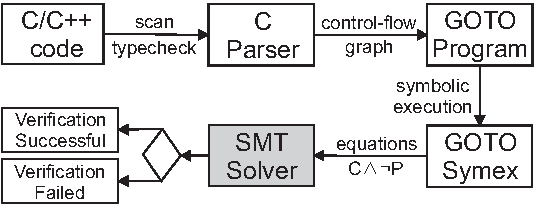
\includegraphics[scale=0.9]{Image/esbmc-arch-new.pdf} 
	\caption{ESBMC Architecture}
	\label{ESBMC-Architecture}
\end{figure}

%----------------------------------------------
\subsection{OpenMP}
\label{OpenMP}
%----------------------------------------------

The OpenMP is a set of directives for parallel programming that augments C/C$++$ and Fortran languages. OpenMP supports most processor architectures and operating systems, {\it e.g.}, Solaris, AIX, HP-UX, Linux, Mac OS X, and Windows. OpenMP uses a portable and very robust model that makes easy for programmers to develop parallel applications for a variety of platforms. 

In particular, OpenMP uses the fork-join model of parallel execution ~\cite{OpenMP1998}. The main thread executes the sequential parts of the program; if a parallel region is encountered, then it forks a team of worker threads. After the parallel region finishes ({\it i.e.}, the API waits until all threads terminate), then the main procedure returns to the single-threaded execution mode~\cite{Wu2014}.

The most basic directive of OpenMP is the ``\#pragma omp parallel for'', which parallelizes the enclosing loop; a basic OpenMP example is shown below:

\begin{lstlisting}[caption=OpenMP basic sample]
01.  int i;
02.  #pragma omp parallel for
03.  for (i = 0; i < 10; i++)
04.      a[i] = 2 * i;
\end{lstlisting}

In the above example, the for loop is executed in parallel. Each iteration of the loop is executed in a separated thread; and each thread may use an idle processor. There is also a way to specify critical regions, which is a code block that is guaranteed to be executed by a single thread at a time. To create a critical region, the ``\#pragma omp critical'' directive should be used.
%----------------------------------------------
\subsection{Solving Optimization Problems with Vz}
\label{Optimization-with-Vz}
%----------------------------------------------

SMT decides the satisfiability of first-order formulas using a combination of different background theories and thus generalizes propositional satisfiability by supporting uninterpreted functions, linear and nonlinear arithmetic, bitvectors, tuples, arrays, and other decidable first-order theories. In this study, the SMT solver Z3 is used to check for the satisfiability of formulas generated from the HW-SW partitioning problem~\cite{Bjorner2014}. In particular, we exploit the use of vZ, which is implemented on top of the SMT solver Z3, in order to solve optimization problems; Vz base function is to optimize objective functions, which formulate optimized criteria, within the logical context of constraints.~vZ also includes an incremental version of the Maximum Resiliency (MaxRes) \cite{Federica2008} in order to achieve Maximum Satisfiability (MaxSAT) \cite{NarodytskaN} and a Simplex to solve numbers without defined patterns. In Vz, MaxSAT is responsible for the restrictions, while OptSMT optimizes linear arithmetic objectives~\cite{Bjorner2015}. In summary, Vz provides three main functions that extend Z3 for solving optimization problems, which are: \textit{maximize}, \textit{minimize}, and \textit{assert-soft}.

\begin{itemize}
\item{\textbf{maximize(T)}
this function informs to the solver that a given variable $T$ should be maximized, which includes real, integer, or bit-vector variables.}
\item{\textbf{minimize(T)}
this function informs the solver that a given variable $T$ should be minimized, the accepted types are the same as maximize function.}
\item{\textbf{Assert-Soft F : weight n}
the function \textit{assert-soft} adds a restriction to $F$, which can also add a weight $n$; the default value is $1$.}
\end{itemize}

As an example, one can optimize $\left(K + W\right)$, with restrictions in $\left(K < 2\right)$ and $\left(W - K < 1\right)$. The expected result of this optimization problem described in the code below is $2$. In fact, the model generated by vZ shows that $K = 1$ and $W = 1$.

\begin{lstlisting}[caption=Example of SMT formula using vZ, label=vZ]
1. (declare-const K Int) 
2. (declare-const W Int)
3. (assert (< K 2)) 
4. (assert (< (- W K) 1))
5. (maximize (+ K W)) 
6. (check-sat)
\end{lstlisting}

The vZ architecture is shown in Fig.~\ref{vZ-Architecture}. Initially, the SMT formula with objectives is converted to $0-1$ constraints, which leads to a Pseudo-Boolean Optimization (PBO)~\cite{Barth1995,Vasco2005}. If there are many objective functions, vZ invokes OptSAT for arithmetic or MaxSAT for soft constraints. For constraints using real values, Vz combines linear arithmetic objectives and uses only one instance of OptSMT. When ``soft constrains'' is used in the mode `` lexicographic'', vZ invokes MaxSAT using multiple calls for its engine.
%
\begin{figure}[ht]
	\centering
  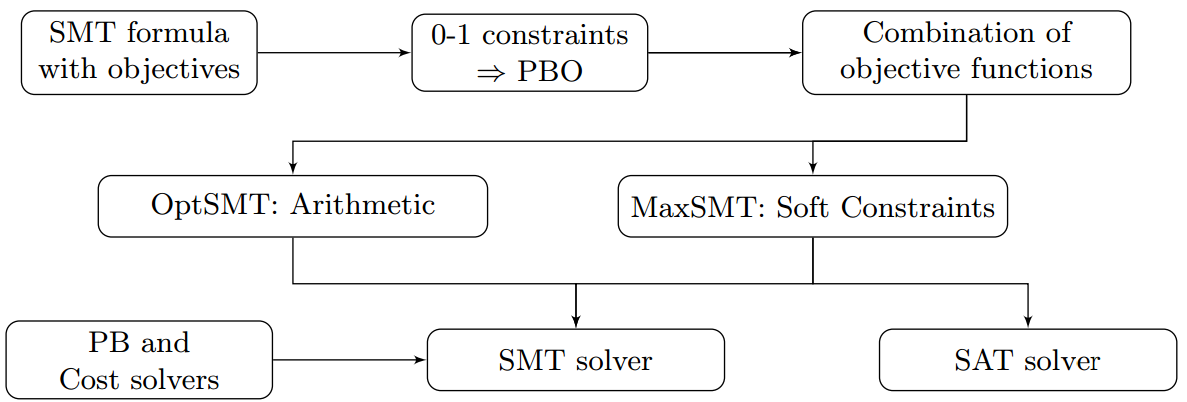
\includegraphics[width=0.49\textwidth, height=95px]{Image/vzArch.png} 
	\caption{vZ Architecture~\cite{Bjorner2015}}
	\label{vZ-Architecture}
\end{figure}

Z3 is available for platforms in C, C$++$, Java, .NET, and Python; it is possible to download Z3 with vZ from its github repository~\cite{Z3API}. In this work, the python API is used to formulate HW-SW partitioning problems using the vZ tool. 

%----------------------------------------------
\section{Mathematical modeling}
\label{Mathematical-modeling}
%----------------------------------------------

The mathematical modeling of the HW-SW partitioning problem was taken from~\cite{Arato2003,Mann2007}.

%----------------------------------------------
\subsection{Informal Model (or Assumptions)}
\label{Informal-Model-or-Assumptions}
%----------------------------------------------

The informal model can be described by five characteristics. First, there is only one software context, i.e., there is just one general-purpose processor, and there is only one hardware context. The components of the system must be mapped to either one of these two contexts. Second, the software implementation of a component is associated with a software cost, which is the running time of the component. Third, the hardware implementation of a component has a hardware cost, which can be area, heat dissipation, and energy consumption. Fourth, based on the premise that hardware is significantly faster than software, the running time of the components in hardware is considered as zero. Finally, if two components are mapped to the same context, then there is no overhead of communication between them; otherwise, there is an overhead. The consequence of these assumptions is that scheduling does not need to be addressed in this work. Hardware components do not need scheduling, because the running time is assumed to be zero. Because there is only one processor, software components do not need to be scheduled as well. Therefore, the focus is only on the partitioning problem. That configuration describes a first-generation co-design, where the focus is on bipartitioning ~\cite{Teich2012}.

%----------------------------------------------
\subsection{Formal Model}
\label{Formal-Model}
%----------------------------------------------

The inputs of the problem are: a directed simple graph $ G = (V,E) $, called the task graph of the system, is necessary. The vertices $V = \{V_1,V_2,\dotso,V_n\}$ represent the nodes that are the components of the system that will be partitioned. The edges $E$ represent communication between components. Additionally, each node  $V_i$ has a cost $h(V_i)$ (or $h_i$) of hardware if implemented in hardware and a cost $s(s_i)$ (or $ s_i $) of software if implemented in software. Finally, $c(V_i,V_j)$ represents the communication cost between $V_i$ and $V_j$ if they are implemented in different contexts (hardware or software).

Based on Arat\'o {\it et al.}~\cite{Arato2003}, is called a hardware-software partition if it is a bipartition of $V:P = (V_h, V_s)$, where $V_h \cup V_s = V$  and $V_h \cap V_s = 0$. The crossing edges are $E_p = \{(V_i,V_j):V_i \in V_s, V_j \in V_h$ or $v_i \in V_h, v_j \in V_s $. The hardware cost of $P$ is given by Eq.~\ref{hardware-costs}
%
\begin{align}
\label{hardware-costs}
H_p  &= \Sigma_{v_i \in V_H} h_i
\end{align}
%
\noindent and the software cost of $P$ ({\it i.e.}, software cost of the nodes and the communication cost) is given by Eq.~\ref{software-communication-costs}
%
%  S_p &= \Sigma_{\left(v_i \;\in\; V_s\right)} s_i + \Sigma_{(v_i,v_j) \in\; %E_p}\; c(V_i, V_j).
\begin{align}
\label{software-communication-costs}
  S_p &= \Sigma_{v_i \in V_s}\:s_i + \Sigma_{(v_i,v_j)\in\:E_p} c(V_i,V_j)
\end{align}

Three different optimization and decision problems can be defined. In this paper, the focus is on the case that $ S_0 $ is given, i.e., to find a $P$ HW-SW partitioning so that $ S_p \leq S_0 $ and $ H_p $ is minimal ({\it i.e.}, system with hard real-time constraints). Based on Equations~\ref{linear-programming-problem} and~\ref{software-communication-costs}, the constraints can be reformulated as 
%
\begin{align}
\label{hw-sw-partitioning}
s\left(1-x\right) + c|E_x| \leq S_0, 
\end{align}
%
\noindent where $x$ represents the decision variable. Concerning the complexity of this problem, Arat\'o {\it et al.}~\cite{Arato2003} demonstrate that it is NP-Hard~\cite{Cormem}.

%----------------------------------------------
\section{Partitioning problem using ILP-based,Genetic Algorithms}
\label{ILPGA}
%----------------------------------------------

The ILP and GA were taken from our previous studies~\cite{Trindade2015,Trindade2014}. Both use slack variables in order to be possible to represent constraints and to use commercial tools. However, GA had improvements from the parameters of related studies in order to increase the solution accuracy without producing timeout. The tuning was performed by empirical tests and resulted in changing of three parameters, which are passed to the function \textit{ga} of MATLAB~\cite{TheMathWorks2013}: the population size was set from $300$ to $500$, the Elite count changed from $2$ (default value) to $50$, and the number of generations changed from $100*NumberOfVariables$ (default) to $75$.

%----------------------------------------------
\section{Analysis of the partitioning problem using vZ}
\label{Analysis-of-the-partitioning-problem-using-vZ}
%----------------------------------------------

Algorithm~\ref{vZ-pseudocode} encodes the objective function and constraints related to the HW-SW partitioning problem using vZ functions~\cite{Bjorner2014}. A vZ logical context must firstly be created (line $02$), in order to add constraints and to check whether a given model exists to the set of constraints. Note that the number of nodes and edges, software, hardware, and communications costs as well as the incidence matrix E must also be declared.

The arithmetic expressions from lines $10$ to $12$ represent the constraints described in Eq.~\ref{hw-sw-partitioning}. Here, variable \textit{SC} refers to the software cost, while \textit{CC} denotes the communication cost. In line $12$, the \textit{Fobj} (objective function) is declared, which denotes the product between the hardware cost and the decision variables vector, which contains only Boolean values. \textit{Fobj} should be minimized to obtain the optimal hardware solution. To achieve this, two constraints are imposed to vZ: the first one refers to the sum of the software and communication costs, where the result should be less than $S_0$; and the second one informs to vZ that \textit{Fobj} should be minimized. Finally, the model is checked by Vz and if there is a solution that meets the constraints, then the \textit{Fobj} value is provided.

\begin{lstlisting}[caption=Pseudocode describing vZ,label=vZ-pseudocode, mathescape]
01.#Initialize Variables
02.  Create vZ context 
03.  Create binary vector (x)
04.  Declare number of nodes, edges and $S_{0}$
05.  Declare hardware cost of each node as array (h) 
06.  Declare software cost of each node as array (s)
07.  Declare communication cost of each edge (c)
08.  Declare transposed incidence matrix graph G (E)
09.#Arithmetic Expressions
10.  SC = s(1-x)
11.  CMC = c*|EX|
12.  Fobj =  x[i] * h[i]
13.#Assert Constraints
14.  Add constraints (SF + CMC <= $S_{0}$)
15.  Add constraints to minimize Fobj
16.  Check Model
17.  Print Result
\end{lstlisting}

%----------------------------------------------
\section{Analysis of the partitioning problem using ESBMC}
\label{Analysis-of-the-partitioning-problem-using-ESBMC}
%----------------------------------------------

As computer hardware architecture moves from single- to multi-cores, parallel programming environments should be exploited to take advantage of the ability to run several threads on different processing cores. This section describes the verification algorithm using sequential ESBMC, followerd by three multi-core model checking algorithms, in order to speed up the HW-SW partitioning verification if compared to the sequential solution.

%----------------------------------------------
\subsection{Verification Algorithm using Sequential ESBMC}
\label{Verification-Algorithm-using-ESBMC}
%----------------------------------------------

ESBMC pseudocode shows the algorithm with the same constraints and conditions placed on ILP and GA. Two values must be controlled to obtain the results and to perform the optimization. One is the initial software cost, as defined in Section~\ref{Formal-Model}. The other is the halting condition (code violation) that stops the algorithm.

The ESBMC algorithm starts with the declarations of hardware, software, and communication costs. $S_0$ must also be defined, as the transposed incidence matrix and the identity matrix, as typically done in MATLAB. Here, matrices $A$ and $b$ are generated. At that point, the ESBMC algorithm starts to differ from the ILP and GA presented in~\cite{Trindade2015} and~\cite{Trindade2014}.

It is possible to inform to ESBMC with which type of values the variables must be tested. Therefore, there is a declaration to populate all the decision variables $x$ with non-deterministic Boolean values. Those values that change for each test will generate a possible solution and obey the constraints. If this is achieved, then a feasible solution is found and the ASSUME directive is responsible for ensuring the compliance of constrains (i.e.,$A.x \leq b$).

A loop controls the cost of hardware hint, starting with zero and reaching the maximum value considering the case, where all nodes are partitioned to hardware. To every test performed, the hardware hint is compared to the feasible solution. This is accomplished by an \textit{ASSERT} statement at the end of the algorithm, a predicate that controls the halt condition (\textit{true-false} statement). If the predicate is \textit{FALSE}, then the optimization is finished, {\it i.e.}, the solution is found. 

The \textit{ASSERT} statement tests the objective function, {\it i.e.}, the hardware cost, and will stop if the hardware cost found is lower than or equal to the optimal solution. However, if \textit{ASSERT} returns a \textit{true} condition, {\it i.e.}, the hardware cost is higher than the optimal solution, then the model-checking algorithm restarts and a new possible solution is generated and tested until the \textit{ASSERT} generates a \textit{false} condition. When the \textit{false} condition happens at verification-time, the execution code is aborted and ESBMC presents the counterexample that caused the condition to be broken. That is the point in which the solution is presented (minimum HW cost).

In the ESBMC algorithm, which is shown below, it is not necessary to add slack variables, because the modulus operation is kept, which reduces the number of variables to be solved. 

\begin{lstlisting}[caption=Pseudocode describing ESBMC, mathescape]
01. Initialize Variables 
02. Declare number of nodes and edges
03. Declare hardware cost of each node as array (h)
04. Declare software cost of each node as array (s)
05. Declare communication cost of each edge (c)
06. Declare the initial software cost of ($S_{0}$)
07. Declare transposed incidence matrix graph G (E)
08. Define the solutions variable ($X_{i}$ ) as Boolean
09. main {
10.  for TipH = 0 to Hmax do {
11.   populate $X_{i}$ with nondeterministic/test values
12.   Calculate s(1-x)+c|$E_{x}$| and store at variable
13.   Requirement isued by Assume (Variable <= $S_{0}$)
14.   Calculate Hp cost Based on value tested of $X_{i}$
15.   Violation check with Assert($H_{p}$ > TipH)
16.  }
17. }
\end{lstlisting}

%In the multi-core ESBMC algorithm, the only difference is the fact that the value of $ TipH $ and its range is not declared in the algorithm, %as shown in ESBMC Pseudocode. The proposed approach is invoked for each test problem, as follows:
%$ esbmc-parallel <Filename.c> \; <hminvalue> \; <Hmax> $

%Where $ <Filename.c> $ is the optimization problem described in ANSI-C format, $  <hminvalue> $ is the minimum (zero to HW-SW partitioning %problem) and $ <Hmax> $ is the maximum hardware cost for the specified problem.

%Therefore, the algorithm starts different ESBMC instances using different optimization values, in ascending order, for $ Hmax $ in order to %find a violation. If all instances finish and no violation is found, then multi-core ESBMC starts new $ N $ instances. When a violation is %found, it reports time and hardware cost. If multi-core ESBMC tests all the possibilities for the hardware cost and has not found a violation, %then it reports: $ Violation not found $.

%----------------------------------------------
\subsection{Multi-core ESBMC with OpenMP (ESBMC-MC)}
\label{Multi-core-ESBMC-with-OpenMP}
%----------------------------------------------

Typically, ESBMC verification runs are performed only in a single-core. If the processor provides $8$ processing cores, only one is used for the verification and the others remain idle. Thus, there is a significant unused hardware resource during this process. 


To optimize the CPU resources utilization without modifying the underlying SMT Solver, the Open Multi-Processing (OpenMP) library~\cite{Dagum1998} is used in this present work as a front-end for ESBMC.

Fig.~\ref{ESBMC-Multi-core} shows our first approach called ``Multi-core ESBMC''.
%
\begin{figure}[ht]
	\centering
  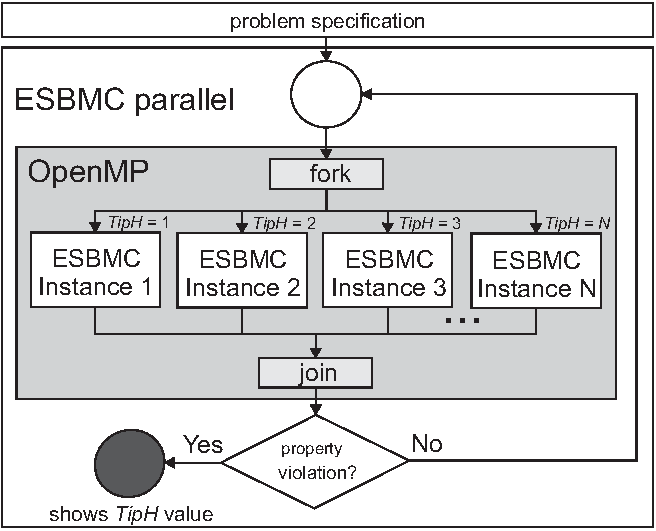
\includegraphics[scale=0.75]{Image/esbmc-parallel.pdf} 
	\caption{ESBMC Multi-core.}
	\label{ESBMC-Multi-core}
\end{figure}

Multi-core ESBMC obtains the problem specification represented by a C program. The HW-SW partitioning is violated, when the correct optimum value (\textit{TipH}) parameter is reached; Multi-core ESBMC starts a parallel region with different instances of ESBMC, based on the number of available processing cores. All these ESBMC instances run independently of each other, as shown in Fig.~\ref{ESBMC-Multi-core}. Note that there is no shared-memory (or message-passing) mechanism among the threads. In particular, different threads are managed by the OpenMP API, which is responsible for the thread lifecycle: start, running, and dead states, using different values as condition. After executing $N$ instances, if there is no code violation, then multi-core ESBMC starts new instances again. During the parallel region execution, if a violation is found in any running thread, then it presents the counterexample with the violation condition and the verification time. If all threads of the batch processing are terminated, then multi-core ESBMC finishes its execution.

%----------------------------------------------
\subsection{Multi-core ESBMC with OpenMP using Workers (ESBMC-PS)}
\label{Multi-core-ESBMC-with-OpenMP-using-workers}
%----------------------------------------------

The previous parallelization is implemented by continuously forking ESBMC instances until the first violation is found. However, since OpenMP only returns from a parallelized loop, when every forked thread finishes, some processing cores could remain idle for some period of time.

\begin{figure}[ht]
	\centering
  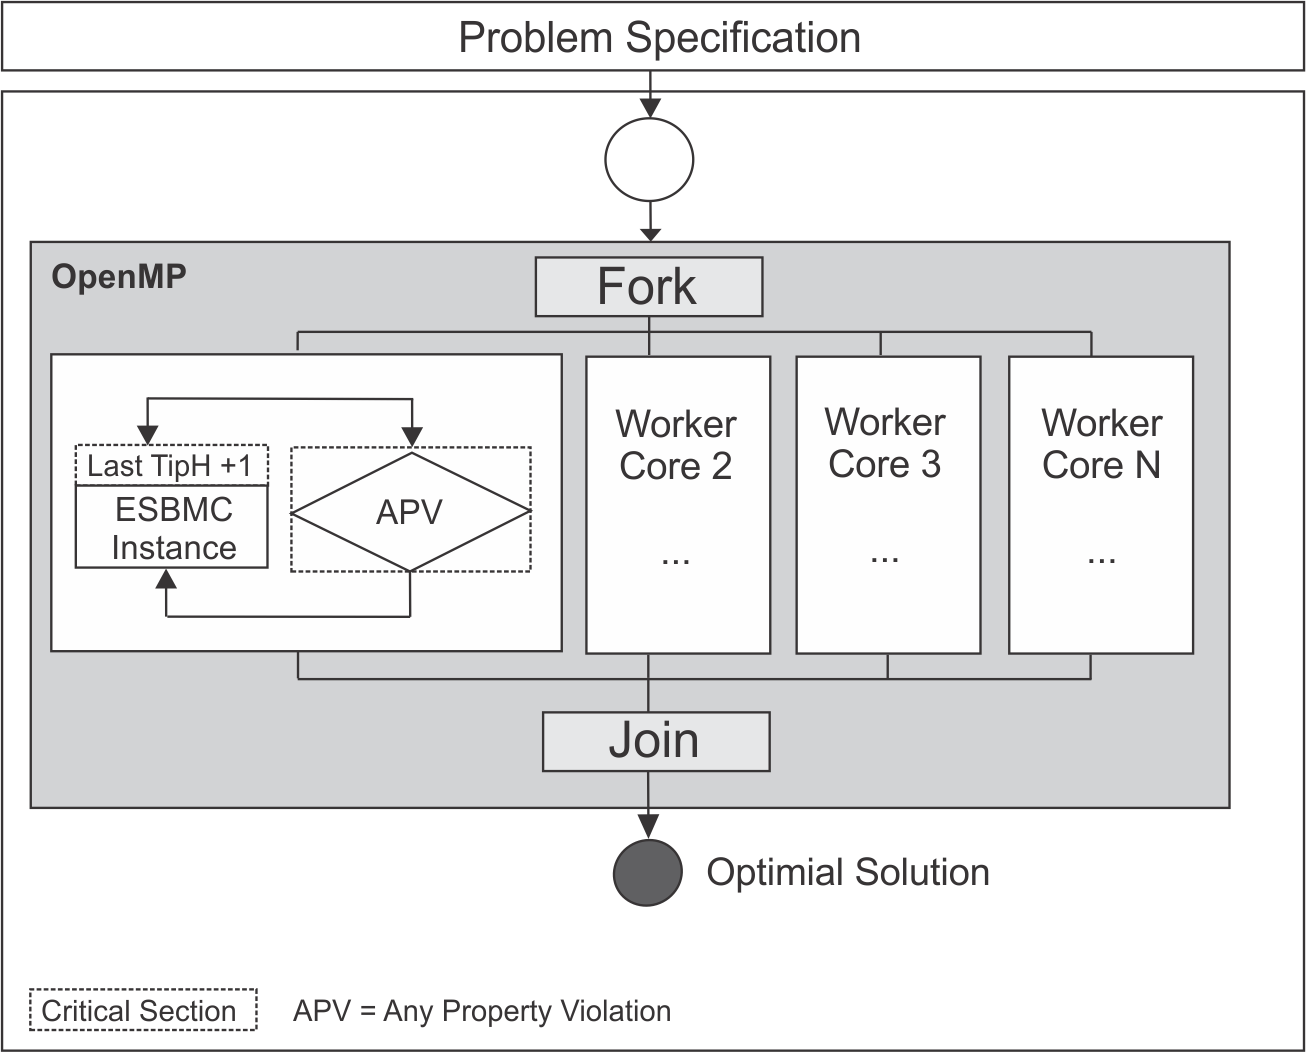
\includegraphics[scale=0.75]{Image/esbmc-parallel.png} 
	\caption{ESBMC Multi-core Optimized Sequential Approach. }
	\label{ESBMC-Multi-core-Optimized-Sequential-Approach}
\end{figure}

Consequently, the second approach aims to remove the idle time from the parallel loops, by creating workers inside threads so that the next step is immediately executed if there is a processing core available. This approach could potentially lead to great performance improvements, but as ESBMC checks for each step almost at the same rate, the processor does not remain idle for a longer period and thus there is almost no optimization.

%----------------------------------------------
\subsection{Multi-core ESBMC with OpenMP using Binary Search (ESBMC-PB)}
\label{Multi-core-ESBMC-with-OpenMP-using-Binary-Search}
%----------------------------------------------

The most optimized approach applies a parallelized binary search to reduce the amount of steps to be executed in order to find the optimal solution. A controller is designed to return the step to be executed so that the number of verification runs are substantially reduced as much as possible. The parallelized binary search accomplishes this by splitting the domain of possible values into intervals and then by returning the middle of the largest interval so that two new intervals are created.
%
\begin{figure}[ht]
	\centering
  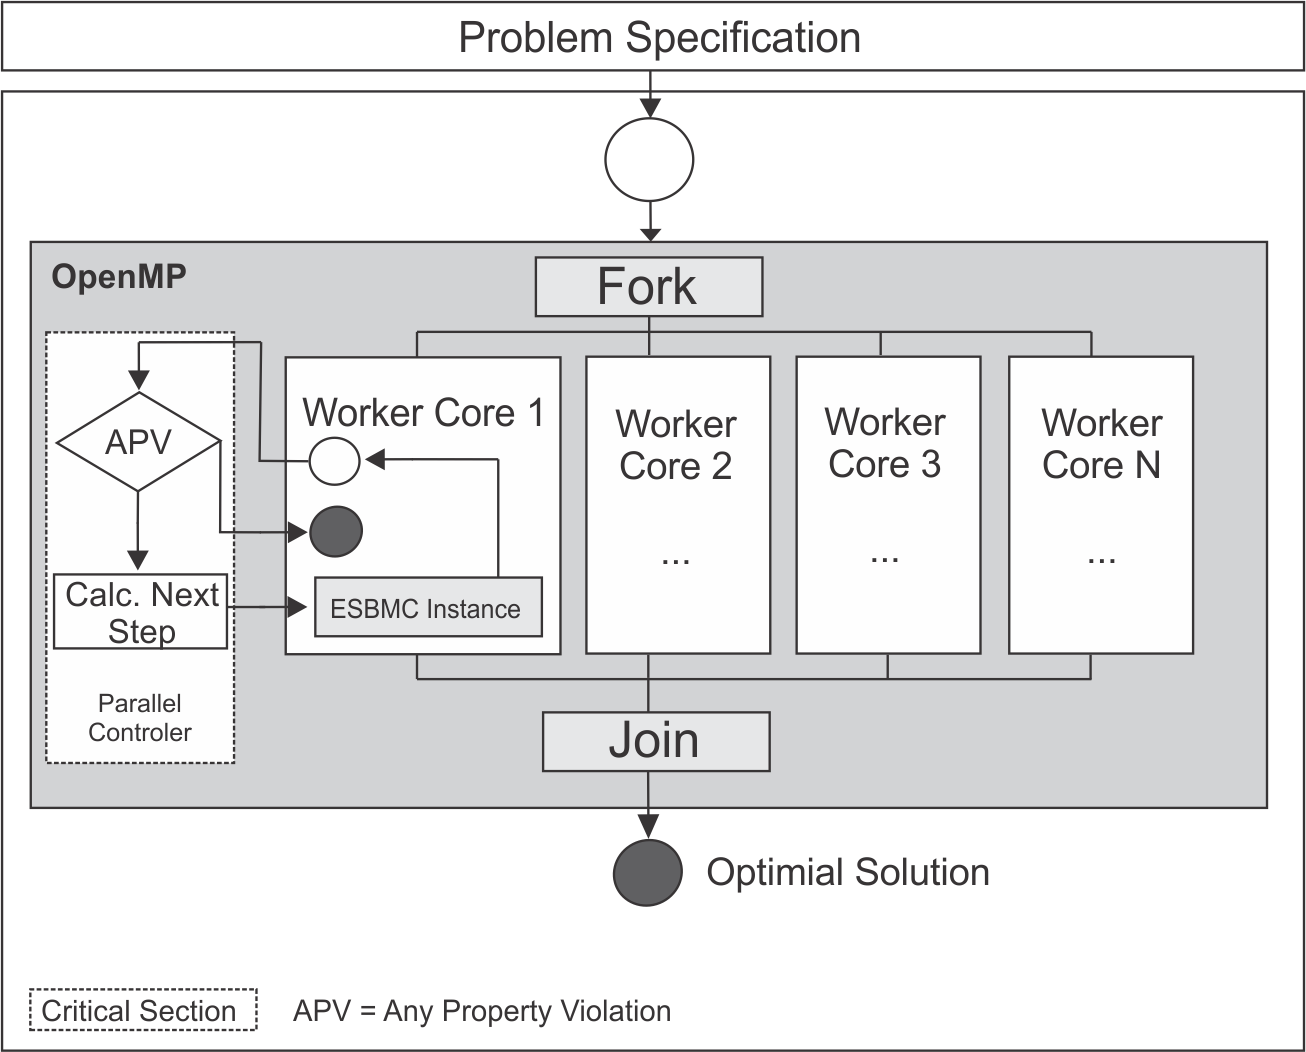
\includegraphics[scale=0.75]{Image/esbmc-parallel-Controler.png} 
	\caption{ESBMC Binary Approach}
	\label{ESBMC-Binary-Approach}
\end{figure}

As an example, given a problem of domain from $1$ to $20$ (see Fig.~\ref{Binary-Step-Calculation}), we firstly create an initial interval from $1$ to $20$. When the next available core asks for a step to be executed, the controller obtains the largest interval ({\it i.e.}, $\left[1,20\right]$, divides it by two, which creates two new intervals ({\it i.e.}, $\left[1,9\right]$ and $\left[11,20\right]$), and returns the middle of the original interval ({\it i.e.}, $10$). The controller also checks whether an interval has less than two elements to avoid creating empty or invalid intervals.
%
\begin{figure}[ht]
	\centering
  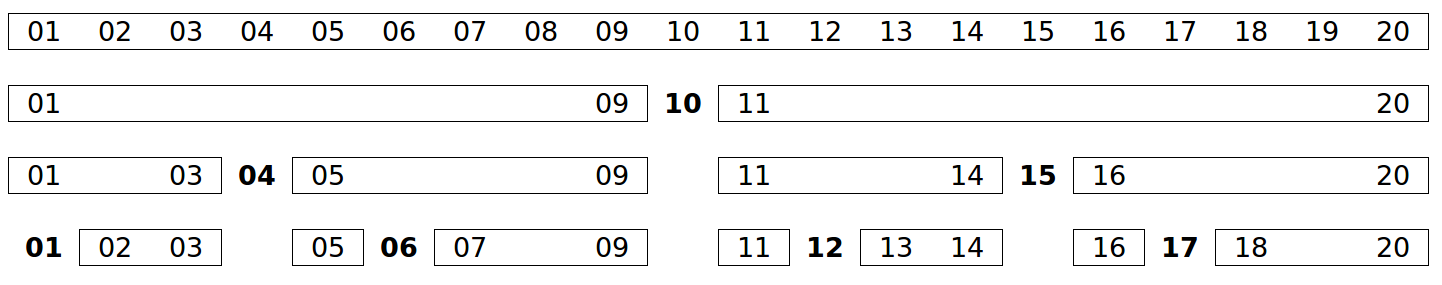
\includegraphics[width=0.49\textwidth, height=75px]{Image/Fig4.png}
	\caption{Binary Step Calculation}
	\label{Binary-Step-Calculation}
\end{figure}

Note that there might gaps between steps, which are produced by the customized binary search. For instance, in the example shown in~\ref{Binary-Step-Calculation}, if step $10$ returns \textit{false}, then one can conclude that all steps after $10$ is \textit{false} as well. However, if the same step $10$ returns \textit{true}, we can assume that all steps before $10$ is \textit{true} as well. As a result, an auxiliary method to remove unnecessary steps is implemented in the controller by removing or shrinking existing intervals. This approach leads to a high impact in the verification time. However, if a step is running and is not needed anymore, the worker kills the forked process and starts a new one.

Note that Algorithm~\ref{Steps-Calculation-using-Intervals} is called from each worker in order to get the next step to execute if it exists; otherwise, either zero or a negative number is returned.

\begin{lstlisting}[caption=Steps Calculation using Intervals,label=Steps-Calculation-using-Intervals]
01. GetNextStep(){
02.  int largestChunk = -1;
03.  chunk largest;
04.  for each(chunk in chunks){
05.     if(chunk.right - chunk.left > largestChunk){
06.           largestChunk = chunk.right - chunk.left;
07.           largest = chunk;
08.     }
09.   }	
10.   chunks.remove(largest);	
11.   int median = largest.left + floor((largest.right - largest.left) / 2)
12.   if(median > 0){
13.      if(largest.right - largest.left > 1)
14.         chunks.add(new chunk(largest.left, median - 1));	
15.      if(largest.right != largest.left)
16.         chunks.add(new chunk(median + 1, largest.right);
17.    }
18.   return median;
19. }
\end{lstlisting}

Algorithm~\ref{Steps-Calculation-using-Intervals} describes how the customized binary search calculates and returns the step to be executed. From lines $4$ to $9$, the algorithm finds the largest interval. Then, from the line $10$ the largest interval is removed and the median is calculated in line $11$. After that, two new intervals are created, the left side (in line $14$) and the right side (in line $16$). At the end, the median is returned.

\begin{lstlisting}[caption=Worker sample,label=worker-sample]
01. step = controller.GetNextStep();
02. int pid = ExecuteStep(step);
03. while(isRunning(pid)){
04.   if(!controller.isNeeded(step))
05.    kill(pid);
06. }     
\end{lstlisting}

Algorithm~\ref{worker-sample} describes how the worker starts and monitors ESBMC instances. The algorithm starts by retrieving the step to be executed from the controller (line $1$), then initiates the ESBMC instance and obtains the process \textit{id} from the forked process (line $2$). While the step is being executed, the controller checks whether this step is still needed (line $4$). If not, then the ESBMC instance is killed (line $5$) and the worker is free to initiate another step.


%----------------------------------------------
\section{Experimental Evaluation}
\label{Experimental-Evaluation}
%----------------------------------------------

This section is split into two parts. The setup is described in Section~\ref{Experimental-Setup} while Section~\ref{Experimental-Results} describes a comparison among Matlab~\cite{TheMathWorks2013}, vZ~\cite{Bjorner2015}, and ESBMC~\cite{Trindade2015} using a set of standard HW-SW partitioning benchmarks~\cite{Mann2007}.

%----------------------------------------------
\subsection{Experimental Setup}
\label{Experimental-Setup}
%----------------------------------------------

To perform the experiments, some test vectors provided by Mann {\it et al.}~\cite{Mann2007} are used, as shown in Table~\ref{Description-of-Benchmarks}. The vertices in the graphs correspond to high-level language instructions. Software and communication costs are time dimensional, and hardware costs represent the occupied area. The first three benchmarks are extracted from MiBench~\cite{Guthaus2001}. The clustering and fuzzy test vectors benchmarks are designed from Mann et al.~\cite{Mann2007} and are significantly larger benchmarks. From the same authors,  very complex benchmarks to test the limits of the applicability of techniques are collected (RC$6$ and Mars).

\begin{table}[h]
\caption {Description of Benchmarks}
\small
\sffamily\footnotesize
\tabulinesep=6pt
\begin{tabular}[c]{m{1.5cm}m{0.8cm}m{0.8cm}m{3.8cm}}
  \toprule[1.5pt]
  \head{Name} & \head{Nodes} & \head{Edges} & \head{Description}\\
  \midrule
  
\verb|CRC32| & \verb|25| & \verb|32| & \rmfamily 32-bit cyclic redundancy check ~\cite{Guthaus2001}\\
\hline
\verb|Patricia| & \verb|21| & \verb|48| & \rmfamily Routine to insert values in Patricia Tree ~\cite{Guthaus2001}\\
\hline

\verb|Dijkstra| & \verb|26| & \verb|69| & \rmfamily Computer shortest paths in a graph ~\cite{Guthaus2001}\\
\hline
\verb|Clustering| & \verb|150| & \verb|331| & \rmfamily Image segmentation algorithm in a medical application\\
\hline
\verb|RC6| & \verb|329| & \verb|448| & \rmfamily RC6 cryptography graph algorithm\\
\hline
\verb|Fuzzy| & \verb|261| & \verb|422| & \rmfamily Clustering algorithm based on fuzzy logic\\
\hline
\verb|Mars| & \verb|417| & \verb|600| & \rmfamily MARS cipher from IBM algorithm\\
 
  \bottomrule[1.5pt]
\end{tabular}
\label{Description-of-Benchmarks}
\end{table}

ESBMC $1$.$24$ running on a $64$-bit Ubuntu $14$.$04$.$1$ LTS operating system was used. A parallel approach of the ESBMC sequential ascending, descending, and binary search are implemented in C++$11$. Version $2$.$0$.$1$ of Boolector SMT-solver~\cite{Brummayer2009} (freely available) was used as the default solver for ESBMC. For ILP and GA formulations, MATLAB R$2013$a from MathWorks with Parallel Computing Toolbox was used~\cite{TheMathWorks2013}. MATLAB is a dynamically typed high-level language known as the state-of-the-art mathematical software~\cite{Tranquillo2011} and is widely used by the engineering community~\cite{Hong2010}. vZ as a built-in tool to Z3 was also used~\cite{Bjorner2014}. 

A desktop with $24$GB of RAM and i$7$ ($8$-cores) from Intel with CPU clock of $3$.$40$ GHz was used. Each time was measured $3$ times in GA (average taken) and just once in vZ, ESBMC, and ILP. The reason is that GA times are not so close as ILP, vZ, and ESBMC. A time out condition (TO) is reached when the running time is longer than $7200$ seconds. A memory out (MO) occurs when the tool reaches $24$GB of memory. 


%----------------------------------------------
\subsection{Experimental Results}
\label{Experimental-Results}
%----------------------------------------------

ESBMC implement four approaches: ESBMC, ESBMC Multicore (MC), ESBMC Parallel Sequential (PS), and ESBMC Parallel binary (PB).

\begin{itemize}
\item{\textbf{ESBMC:} This strategy uses only one core to solve the partitioning problem, as described in Section~\ref{Verification-Algorithm-using-ESBMC}.
\item{\textbf{ESBMC-MC:} This uses a sequential strategy \{1 ,2 ,\:...\:, Hmax\}; there is no parallel controller in this approach, as described in Section~\ref{Multi-core-ESBMC-with-OpenMP}.}
\item{\textbf{ESBMC-PS:} This approach is similar to ESBMC MC; however, it uses a more optimized way to launch the ESBMC instances, as described Section~\ref{Multi-core-ESBMC-with-OpenMP-using-workers}.}
\item{\textbf{ESBMC-PB:} This strategy uses a parallel binary search, as described in Section~\ref{Multi-core-ESBMC-with-OpenMP-using-Binary-Search}.}}
\end{itemize}

There is no single tool for efficiently solving all HW-SW partitioning benchmarks. In particular, Vz solves $4$ out of $7$ benchmarks, but it does not find the optimal solution for the RC$6$ benchmark; vZ is typically faster than ILP by approximately $3$ times ({\it e.g.}, Patricia benchmark); however, vZ returns two TOs (time-outs) in Fuzzy and Mars benchmarks.

In contrast to vZ, ILP solves $6$ out of $7$ benchmarks. When ILP produces a result, it always provides the optimal solution. On the one hand, ILP execution time is slower than vZ in all benchmarks, which are supported by vZ. On the other hand, ILP is faster than ESBMC in all benchmarks, except for the clustering.

Note that all ESBMC parallel versions produce better results than the sequential one. In particular, the ESBMC-PB implementation outperforms all other ESBMC approaches; the ESBMC-PB performance improves as the number of nodes and edges increase. One notable case is the clustering benchmark, when verified by ESBMC-PB, it executes $3$.$13$ times faster than ILP and $1$.$89$ times slower than vZ.

\textcolor{red}{The ESBMC-PB implementation described in Section~\ref{Multi-core-ESBMC-with-OpenMP-using-Binary-Search} shows a significant performance improvement; when the amount of nodes is around $30$, ESBMC-PB does not outperform the optimization techniques employed by vZ and ILP tools. However, when the amount of nodes is approximately $150$, ESBMC-PB becomes three times faster than ILP, which is the most robust technique. When vZ explores a small amount of nodes, it is typically $30$ times faster ({\it e.g.}, CRC$32$) than ESBMC-PB and for intermediate nodes (around $150$ nodes), this performance improvement decreases to $1$.$9$ ({\it e.g.}, Clustering). When analyzing all benchmarks: RC$6$, Fuzzy, and Mars, ESBMC-PB produces TO or MO; however, the results are still promising if we take into consideration that vZ and Matlab are state-of-the-art tools with respect to optimization problems.}

The only technique that is able to solve all benchmarks is GA; however, its precision is not satisfactory since it produces an error rate between $-37.6$\% and $29.0$\%.

Table~\ref{Experimental-results-of-the-complex-benchmarks} shows the experimental results using vZ, Matlab (ILP and GA), and ESBMC (ESBMC\hyp{}MC, ESBMC\hyp{}PS, ESBMC\hyp{}PB) tools.

RC$6$ produced time out for all versions of ESBMC, vZ e GA did not produce the correct answer, and ILP solves correctly all benchmarks, except one. Fuzzy produced time-outs and memory-outs in all tools. ILP was the only one to solve Mars, while GA solved incorrectly all benchmarks.

Clustering described in Table~\ref{Experimental-results-of-the-complex-benchmarks} seems to be the limit to test the described tools, note that more than $150$ nodes lead to TO and MO. ILP shows robustness and produces results even for a high amount of nodes and edges.

\begin{table*}[t]
  \centering
  \caption{Experimental results of the complex benchmarks}  
  \begin{tabular}{*{9}{cc|c|c|c|c|c|c|c}}

 &  & \textbf{CRC32} & \textbf{Patricia} & \textbf{Dijkstra} & \textbf{Clustering} & \textbf{RC6} & \textbf{Fuzzy} & \textbf{Mars} \\[0.15cm]
\cmidrule(r){3-9}

&\textbf{Nodes} &25 &21 &26 &150 &329 &261 &417\\
&\textbf{Edges} &32 &48 &69 &331 &448 &442 &600\\
&\textbf{S0} &20 &10 &20 &50 &600 &4578 &300\\

%EXACT Solution
\bottomrule[1.5pt]
\rowcolors{1}{}{lightgray}

\multirow{2}{*}{\textbf{Exact Solution}}
&  Hp   &  15   &  47   &  31   &  241   &  692    &  13820   &  876 \\
&  Sp   &  19   &  4   &  19   &  46   &  533    &  4231   &  297  \\


%vZ
\bottomrule[1.5pt]
\multirow{2}{*}{\textbf{vZ}}
&  T(s)   &  0.2   &  0.3   &  0.6   &  109   &  112    &  TO   &  TO  \\
&  Hp   &  15   &  47   &  31   &  241   &  241    &  -   &  -  \\
\hline

%ILP
\multirow{2}{*}{\textbf{ILP}}  
&  T(s)   &  2   &  1   &  2   &  649   &  1806    &  TO   &  5.42  \\
&  Hp   &  15   &  47   &  31   &  241   &  692    &  -   &  876  \\
\hline

%GA
\multirow{2}{*}{\textbf{GA}}
&  T(s)   &  7   &  7   &  9   &  340   &  2050    &  1.37   &  5000  \\
&  Error \%   &  13.3   &  0   &  29   &  1.7   &  -6.5    &  -37.6   &  -27.5  \\
\hline

%ESBMC
\multirow{2}{*}{\textbf{ESBMC}}
&  T(s)   &  31   &  362   &  292   &  3010   &  TO    &  MO   &  MO  \\
&  Hp   &  15   &  47   &  31   &  241   &  -    &  -   &  -  \\
\hline

%MultiCore ESBMC
\multirow{2}{*}{\textbf{ESBMC-MC}}
&  T(s)   &  2   &  6   &  7   &  1615   &  TO    &  TO   &  TO  \\
&  Hp   &  15   &  47   &  31   &  241   &  -    &  -   &  -  \\
\hline

%ESBMC Parallel sequential
\multirow{2}{*}{\textbf{ESBMC-PS}}
&  T(s) &  4 &  10   &  11   &  2238   &  TO    &  MO   &  MO  \\
&  Hp   &  15   &  47   &  31   &  241   &  -    &  -   &  -  \\
\hline

%ESBMC Parallel Binary
\multirow{2}{*}{\textbf{ESBMC-PB}}
&  T(s)   &  6   &  5   &  6   &  207   &  TO    &  MO   &  MO \\
&  Hp   &  15   &  47   &  38   &  241   &  -    &  -   &  -  \\
\bottomrule[1.5pt]
\end{tabular}
\label{Experimental-results-of-the-complex-benchmarks}
\end{table*}

%----------------------------------------------
\section{Related Work}
\label{Related-Work}
%----------------------------------------------

Since the second half of the first decade of the 2000s, three main paths have been tracked to improve or to present alternative solutions to the optimization of HW-SW partitioning, {\it i.e.}, to find the exact solution ~\cite{Mann2007}, to use heuristics to speed up performance time ~\cite{Arato2003}, and hybrid ones ~\cite{Arato2005}.

In the first group, the exact solution to the HW-SW partitioning problem is found. The use of SMT-based verification presented in this paper can be grouped into this category, because the exact solution is found with the given algorithm. The difference is based only in terms of the technique chosen to solve the problem.
Another path followed in past initiatives and which has had more studies is the creation of heuristics to speed up the running time of the solution. The difference between this kind of solutions and SMT-based verification is based on two facts: ESBMC is guaranteed to find the exact solution, but the heuristics are faster when the complexity is greater.

Finally, there are approaches that mixes heuristics with exact solution tools. The idea is to use a heuristic to speed up some phase of an exact solution tool. It worth mentioning that the final solution is not necessarily an optimal global solution. Only the SMT-based verification is guaranteed to find the exact solution, but hybrid algorithms are faster when complexity rises.

In terms of SMT-based verification, most work is restricted to present the model, its modification to programming languages ({\it e.g.}, C/C++ and Java), and the application to multi-thread algorithms or to embedded systems to check for program correctness. In ~\cite{Ramalho2013} it presents a bounded model checker for C++ programs, which is an evolution of dealing with C programs and ~\cite{Cordeiro2012} uses the ESBMC model checker for embedded ANSI-C software. In~\cite{Trindade2015} and~\cite{Trindade2014} it was proven that it is possible to use ESBMC to solve HW-SW partitioning, but in a single core way. There are related studies focused on decreasing the verification time of model checkers by applying Swarm Verification ~\cite{Holzmann2011}, and modifications of internal search engines to support parallelism ~\cite{Holzmann2012}, but there is still the need for initiatives related to parallel SMT solvers ~\cite{Wintersteiger2009}. Recently, the SMT solver Z3 has been extended to pose and solve optimization problems modulo theories ~\cite{Bjorner2015}.

\textcolor{Red}{The vZ tool ~\cite{Bjorner2014} and ~\cite{Bjorner2015} offer substantial improvements on optimization problems. The work described in ~\cite{Pavlinovic2015} reports compiler errors and its confuse messages, the classic approach is to show to the programmer the error location and a hint about it, however, another error sources are not considered, the most appropriate approach would be to consider all possible error sources. To model the problem the restrictions are generated using EasyOCaml, and vZ is responsible to compute the best error path. The algorithm described in ~\cite{Pavlinovic2015} shows efficient against the other approaches.}

\textcolor{Red}{The problem adressed in this work uses a single objective, minimizing of the objective function, in ~\cite{Patrick2015} is compared the tools  OptiMathSAT and vZ for software optimization problems. OptiMathSAT using multiple objectives works way better than vZ, however, for problems with single objectives vZ behaves better than OptiMathSAT.}

%----------------------------------------------
\section{Conclusions}
\label{Conclusions}
%----------------------------------------------

We presented four approaches to solve the HW-SW partitioning problem and compared them to other three state-of-the-art techniques. Experimental results showed that for a number of nodes larger than $300$, the best solution for the HW-SW partitioning problem is ILP. Below that, the best option turns out to be vZ since its execution time is faster and notorious. ESBMC is a viable alternative for a number of nodes lower than $150$.  GA had an intermediate result in terms of performance, but the error presented from exact solution made it not acceptable to that kind of application. This error may be reduced by changing some parameters. 

%The computing time to solve the optimization problem reached some hours of execution on a standard desktop computer. 

If considering off-the-shelf tools, as MATLAB to ILP and GA, the coding is simpler. However, ESBMC and Vz have BSD-Style and MIT licenses, respectively and can be downloaded and used for free. Experimental results also pointed to an improvement of ESBMC, when using a parallel approach. In particular, all three parallel approaches described in this paper produced expressive results. The fastest ESBMC approaches is ESBMC-PB (Parallel Binary), which produces good results for an intermediate amount of edges and nodes. Thus, considering that nowadays processors have more and more cores, when modeling the problem, it is possible to consider multi-core model checking as an alternative to solve the HW-SW partitioning problem. 

Finally, there is an issue about $150$ nodes problem, since it seems to be the limit of ESBMC. It really depends on the modeling granularity of the problem. Some researchers propose fine-grained models, in which each instruction can be mapped to either HW or SW. This may lead to thousands of nodes or even more. Others defend coarse-grained models, where decisions are made for larger components, thus even complex systems may consist of just some dozens of nodes to partition. In principle, a fine-grained approach may allow to obtain better partitions, but at the cost of an exponential increase of the search space size. In future work, we will address improvements in ESBMC to remove the parallel layer on top of ESBMC and implement it during symbolic execution so that we can optimize the overall verification time.

%----------------------------------------------
%\section{References}
%\label{References}
%----------------------------------------------
%%%%%%%%%%%%%%%%%%%%%%%%%%
% ---- Bibliography ---- %
%%%%%%%%%%%%%%%%%%%%%%%%%%

\begin{thebibliography}{5}
\providecommand{\natexlab}[1]{#1}
\providecommand{\url}[1]{{#1}}
\providecommand{\urlprefix}{URL }
\expandafter\ifx\csname urlstyle\endcsname\relax
  \providecommand{\doi}[1]{DOI~\discretionary{}{}{}#1}\else
  \providecommand{\doi}{DOI~\discretionary{}{}{}\begingroup
  \urlstyle{rm}\Url}\fi
\providecommand{\eprint}[2][]{\url{#2}}

%1
\bibitem{Arato2003}
Arat\'o, P., Juh\'asz, S., Mann, Z.A., Orb\'an, A., Papp, D. (2003), ``{Hardware/software partitioning in embedded system design. In: Proc. of the Intl. Symposium of Intelligent Signal Processing},'' pp. 192--202.

%2
\bibitem{Mann2007}
Mann, Z.A., Orb\'an, A., Arat\'o, P., ``{Finding optimal hardware/software partitions. In: Formal Methods in System Design},'' v. 31, n. 3 pp. 241--263.

%3
\bibitem{Baier2008}
Baier, C., Katoen, J-P (2008), ``{Principles of Model Checking}'', The MIT Press, London.

%4
\bibitem{Clarke2009}
Clarke, E., Emerson, E., Sifakis, J. (2009), ``{Model checking: algorithmic verification and debugging. In: Communications of the Association Computing Machinery},'' v. 52, n. 11, pp. 74--84.

%5
\bibitem{Trindade2015}
Trindade, A., Cordeiro. L. (2015), ``{Applying SMT-based verification to hardware/software partitioning in embedded systems. In: Design Automation for Embedded Systems (to appear).}''

%6
\bibitem{Trindade2014}
Trindade, A., Cordeiro, L. (2014), ``{Aplicando Verificação de Modelos para o Particionamento de Hardware/Software. In: Brazilian Symposium on Computing Systems Engineering (SBESC)},'' pp. 1--6.

%7
\bibitem{Wu2014}
Wu, M., Wu, W., Tai, N., Zhao, H., Fan, J., Yuan, N. (2014), ``{Research on OpenMP model of the parallel programming technology for homogeneous multicore DSP. In: Proc. of the Intl. Conference on Software Engineering and Service Science},'' pp. 921--924.

%8
\bibitem{Tang2009}
Tang, T., Lin, Y., Ren, X. (2010), ``{Mapping OpenMP concepts to the stream programming model. In: Proc. Intl. Conference on Computer Science Education (ICCSE)},'' pp. 1900--1905.

%9
\bibitem{Rao2009}
Rao, S. (2009), ``{Engineering Optimization: Theory and Practice. 4th edition}'', John Wiley \& Sons, Hoboken.

%10
\bibitem{Biere2009}
Biere, A. (2009), ``{Bounded model checking. In: Biere, A., Heule, M., van Marren, H., Walsh, T. (org.)}'', Handbook of Satisfiability, IOS Press, pp. 457–-481.

%11
\bibitem{Clarke2004}
Clarke, E., Kroening, D., Lerda, F. (2004), ``{A Tool for Checking ANSI-C Programs. In: Proc. of the Tools and Algorithms for the Construction and Analysis of Systems}'', LNCS 2988, pp. 168--176.

%12
\bibitem{Armando2009}
Armando, A., Mantovani, J., Platania, L. (2009), ``{Bounded model checking of software using SMT solvers instead of SAT solvers. In: International Journal on Software Tools for Technology Transfer},'' v. 11, n. 1, pp. 69--83.

%13
\bibitem{Ganai2006}
Ganai, M., Gupta, A. (2006), ``{Accelerating high-level bounded model checking. In: Proc. of the IEEE/ACM International Conference on Computer-Aided Design},'' pp. 794-–801.

%14
\bibitem{Cordeiro2012}
Cordeiro, L., Fischer, B., Marques-Silva, J. (2012), ``{SMT-based bounded model checking for embedded ANSI-C software. In: IEEE Transactions on Software Engineering},'' v. 38, n. 4, pp. 957--974.

%15
\bibitem{Cordeiro2011}
Cordeiro, L., Fischer, B. (2011), ``{Verifying multi-threaded software using SMT-based context-bounded model checking. In: Proceedings of the 33rd International Conference on Software Engineering},'' pp. 331--340.

%16
\bibitem{Ramalho2013}
Ramalho, M., Freitas, M., Souza, F., Marques, H., Cordeiro, L. (2013), ``{SMT-Based Bounded Model Checking of C++ Programs. In: International Conference and Workshops on the Engineering of Computer-Based Systems},'' pp. 147--156.

%17
\bibitem{Teich2012}
Teich, J. (2012), ``{Hardware/Software Codesign: The Past, the Present, and Predicting the Future. In: Proc. of the IEEE, Special Centennial Issue},''  v. 100, pp. 1411--1430.

%18
\bibitem{TheMathWorks2013}
The MathWorks, Inc. (2013), ``{MATLAB (version R2013a)}'', Natick, MA.

%19
\bibitem{Tranquillo2011}
Tranquillo, J. (2011), ``{Matlab for Engineering and the Life Sciences}'', Synthesis Lectures on Engineering. Morgan \& Claypool.

%20
\bibitem{Hong2010}
Hong, L., Cai, J. (2010), ``{The application guide of mixed programming between MATLAB and other programming languages. In: Proc. of the 2nd Intl. Conference on Computer and Automation Engineering},'' pp. 185--189.

%21
\bibitem{Guthaus2001}
Guthaus, M., Ringenberg, J., Ernst, D., Austin, T., Mudge, T., Brown, R. (2001), ``{MiBench: a free, commercially representative embedded benchmark suite. In: Proc. of the IEEE 4th annual workshop on workload characterization},'' pp. 3--14.

%22
\bibitem{Arato2005}
Arat\'o, P., Mann, Z.A., Orb\'an, A. (2005), ``{Algorithmic aspects of hardware/software partitioning. In: Association Computing Machinery Transactions on Design Automation of Electronic Systems},'' v. 1, pp. 136–-156.

%23
\bibitem{Dagum1998}
Dagum, L., Menon, R. (1998), ``{OpenMP: an industry-standard API for shared-memory programming.},'' In: Computational Science \& Engineering, v. 5, n. 1, pp. 46--55.

%24
\bibitem{DeMoura2008}
De Moura, L., Bjorner, N. (2008), ``{Z3: An Efficient SMT Solver. In: Tools and Algorithms for the Construction and Analysis of Systems},'' LNCS 4963, pp. 337–-340.

%25
\bibitem{Brummayer2009}
Brummayer, R., Biere, A. (2009), ``{Boolector: An Efficient SMT Solver for Bit-Vectors and Arrays. In: Tools and Algorithms for the Construction and Analysis of Systems},'' LNCS 5505, pp. 174-–177.

%26
\bibitem{Barrett2011}
Barrett, C., Conway, C. Deters, M., Hadarean, L., Jovanovic, D., King, T., Reynolds, A., Tinelli, C. (2011), ``{CVC4. In: Computer-Aided Verification},'' LNCS 6806, pp. 171--177.

%27
\bibitem{Bozzano2005}
Bozzano, M., Bruttomesso, R., Cimatti, A., Junttila, T., Rossum, P., Schulz, S., Sebastiani, R. (2005), ``{MathSAT: Tight integration of SAT and mathematical decision procedures},'' In: Journal of Automated Reasoning, v. 35, n. 1-3, pp. 265--293.

%28
\bibitem{Dutertre2014}
Dutertre, B. (2014), ``{Yices 2.2. In: Computer-Aided Verification (CAV)},'' LNCS 8559, pp. 737–-744.

%29
\bibitem{Holzmann2011}
Holzmann, G.J., Joshi, R., Groce, A. (2011), ``{Swarm Verification Techniques},'' In: IEEE Transactions on Software Engineering, v. 37, n. 6, pp. 845--857.

%30
\bibitem{Holzmann2012}
Holzmann, G. (2012), ``{Parallelizing the spin model checker. In: Proc. of the 19th Intl. Conference on Model Checking Software},'' LNCS 7385, pp. 155--171.

%31
\bibitem{Wintersteiger2009}
Wintersteiger, C., Hamadi, Y., De Moura, L. (2009), ``{A Concurrent Portfolio Approach to SMT Solving.},'' In: Proc. of the Intl. Conference on Computer-Aided Verification, LNCS 5643, pp. 715--720.

%32
\bibitem{Bjorner2015}
Bjorner, N., Phan, A-D., Fleckenstein, L. (2015), ``{vZ - An Optimizing SMT Solver},'' In: Proc. of the International Conference on Tools and Algorithms for the Construction and Analysis of Systems, LNCS 9035, pp. 194--199.

%33
\bibitem{Qawasmeh2014}
Qawasmeh, A., Malik, A., Chapman, B. (2014), ``{OpenMP task scheduling analysis via OpenMP runtime API and tool visualization.},'' In: Proc. of the Intl. Parallel \& Distributed processing symposium workshop, pp. 1049--1058.

%34
\bibitem{Bjorner2014}
Bjorner, N. and Phan, A. D. (2014), ``{vZ - Maximal Satisfaction with Z3},'' In: Prof. of the 6th Intl. Symposium on Symbolic Computation in Software Science, pp. 1--10.

%35
\bibitem{OpenMP1998}
OpenMP Architecture Review Board, OpenMP C and C++
Application Pogram Interface, Version 1.0, October 1998.
http://www.openmp.org

%36
\bibitem{Z3API}
Magellan, ``{Source code and documentation},''
  \url{https://github.com/Z3Prover/z3}, Accessed 18th August 2015.
  
%37
\bibitem{GA}
URFJ, ``{Algoritmos Genéticos: Fundamentos e Aplicações. Marcio Nunes de Miranda},''
  \url{http://www.nce.ufrj.br/GINAPE/VIDA/alggenet.htm}, Accessed 18th August 2015.

%38
\bibitem{NarodytskaN}
Narodytska, N., Bacchus, F. (2014), {``Maximum Satisfiability Using Core-Guided MAXSAT Resolution},'' In: Proc. of the Twenty-Eighth AAAI Conference on Artificial Intelligence, pp. 2717--2723.

%39
\bibitem{Federica2008}
Federica, P., Rodolfo, F., Yuqing , S., Elisa, B. (2008), {``Authorization and User Failure Resiliency for WS-BPEL business processes''}, In: Service-Oriented Computing, LNCS 5364, pp. 116--131

%40
\bibitem{Barth1995}
Barth, P., Davis-Putnam, A. (1995), {``Enumeration Algorithm for Linear
Pseudo-Boolean Optimization.''}, Technical Report MPI-I-95-2-003, Max Plank Institute for Computer Science.

%41
\bibitem{Vasco2005}Vasco, M., Marques-Silva, J., {``Effective Lower Bounding Techniques for Pseudo-Boolean Optimization''}, IST/INESC-ID, Technical University of Lisbon, Portugal.

%42
\bibitem{Pavlinovic2015}Pavlinovic, Z., King, T., Wies, T.,{``Practical SMT-Based Type Error Localization''}, ICFP’15, August 31 – September 2, 2015, Vancouver, BC, Canada c 2015 ACM. 978-1-4503-3669-7/15/08

%43
\bibitem{Patrick2015}Sebastiani, R., Trentin, T., {``OptiMathSAT: A Tool for Optimization Modulo Theories''}

%43
\bibitem{Cormem}
Cormen, T., Leiserson, C., Rivest, R., Stein, C. (2009), {``Introduction to Algorithms''}, MIT Press, pp. I-XIX, 1--1292.

\end{thebibliography}

\end{document}


% end of file template.texe os 